
\chapter{Experimental Results}
\label{chap:exp}

This chapter presents the experiments and the results of the evaluations to the propose robot-camera calibration method as well as to the pose estimation system. In addition to those, an evaluation of the accuracy of the cameras used in this thesis is presented. In order to make such evaluation, the reprojection error, a well understood and known metric in the field of computer vision is used. The reprojection error is an import and crucial step which can determine how accurate the robot-camera calibration can be, for that reason it is performed first, followed by the evaluation of the robot-camera calibration which is essential and determinant step to have a good performance in the pose estimation system, which is the last one to undergo an evaluation process as well.

\section{Robot-Camera Calibration on the Yumi robot}
In order to get an accurate estimation of the robot-camera pose depends on how well the estimation of the intrinsic parameters related to the camera can be. Such estimation of those parameters was accomplished as described in section \ref{pppp}, where those existing algorithms were used for checkerboard detection in both colour and depth data. With those parameter knowing in advance, a reprojection error is calculated for both cameras. 

\subsubsection{Reprojection Error}

The reprojection error is the distance between a pattern keypoint detected in a calibration image, and a corresponding world point projected into the same image. Figure \ref{fig:realopen} and Figure \ref{fig:realros} show the calibration results by analyzing the reprojection error per image for the RealSense camera when OpenCV and camera \textunderscore industrial calibration were used. Figure \ref{fig:astraopen} and Figure \ref{fig:astraros} show the calibration results by analyzing the reprojection error per image for the Astra camera when the OpenCV and camera \textunderscore industrial calibration were used.
%%%%%%%%%%%%%%%%%%%%%%%%%%%%%%%%%%%%%%%%%%
\begin{figure}[!h]
\begin{center}
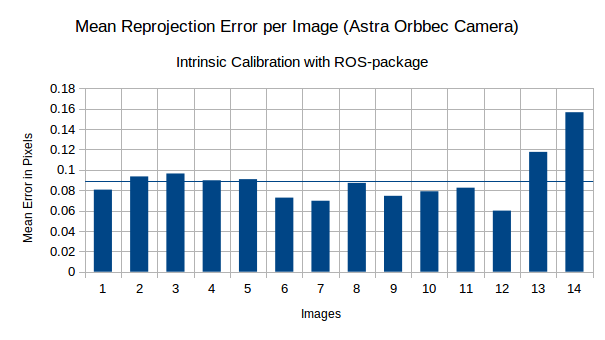
\includegraphics[width=5in, height=3.5in]{figures05/ros_int_cal_astra.png}
\caption{Mean Reprojection Error per image with a ROS method (Astra Orbbec Camera)}%\cite{temp2}}
\label{fig:astraros}
\end{center}
\end{figure}

\begin{figure}[!h]
\begin{center}
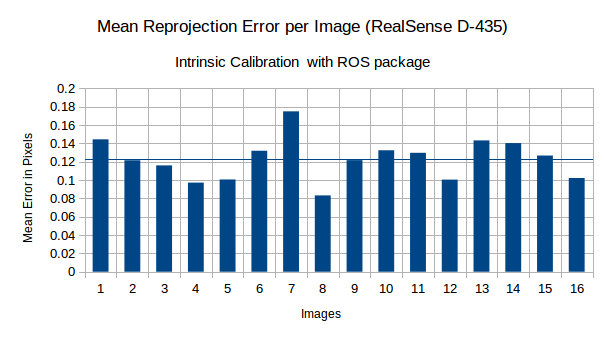
\includegraphics[width=5in, height=3.5in]{figures05/ros_int_cal_real.png}
\caption{Mean Reprojection Error per image with a ROS method (RealSense D-435)}%\cite{temp2}}
\label{fig:realros}
\end{center}
\end{figure}

\begin{figure}[!h]
\begin{center}
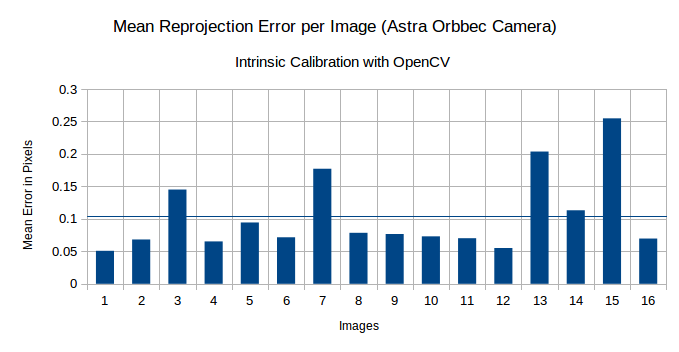
\includegraphics[width=5in, height=3.5in]{figures05/opencv_int_cal_astra.png}
\caption{Mean Reprojection Error per image with a OpenCV method (Astra Orbbec Camera)}%\cite{temp2}}
\label{fig:astraopen}
\end{center}
\end{figure}

\begin{figure}[!h]
\begin{center}
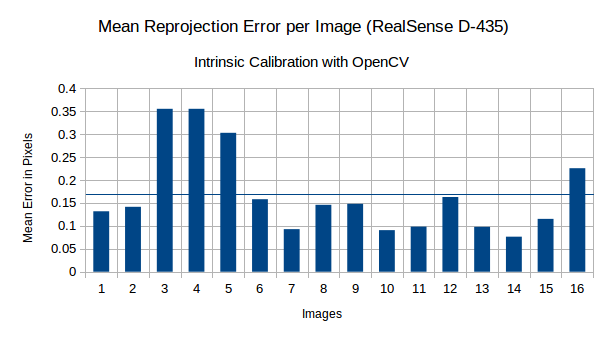
\includegraphics[width=5in, height=3.5in]{figures05/opencv_int_cal_real.png}
\caption{Mean Reprojection Error per image with a OpenCV method (RealSense D-435)}%\cite{temp2}}
\label{fig:realopen}
\end{center}
\end{figure}

To find the average error we calculate the arithmetical mean of the errors calculates for all the calibration images. This should be as close to zero as possible. 

\subsubsection{Result Analysis}
After computing the average error for both cameras, the results are shown in Table \ref{astra1} related to the Astra camera and Table \ref{real1} which corresponds to the RealSense D-435. It can be seen that the overall mean error representing the Astra camera is quite correlated to one another method (OpenCV or camera \textunderscore industrial calibration). The difference is acceptable since it is under the standard specified in most of the literature of computer vision as it is that the error should as close as possible to 0, or under the 0.5 pixels.\\
On the other hand, the results for the RealSense camera are not quite correlated at all. There exists a difference that can affect the eye-to-hand calibration process, and therefore, the pose estimation system can be affected also. Even when the overall mean error meets the requirements of being under the 0,5 pixels, it is difficult to conclude that the RealSense camera is or is not a good choice for solving the main problem of this thesis as it is the pose estimation system. But, it is a good insight to know in advance for future conclusions where there might exist potential issues in the development of this master thesis.
As a remark, both cameras were calibrated with same light conditions, with the same calibration target and with an equal number of images. Considering, all in all, it can be concluded that the Astra camera seems to perform well and it can be our final choice for the pose estimation system.

\begin{table}[b]
% increase table row spacing, adjust to taste
\renewcommand{\arraystretch}{1.3}
\caption{Experiment data for internal Astra sensor calibration.}
\label{astra1}
\centering
\begin{tabular}{|c||c|}
\hline
Method & Overall Mean Error\\
\hline
OpenCV &  0.1041954808\\
\hline
ROS &  0.1081118023\\
\hline
\hline
\end{tabular}
\end{table}

\begin{table}[b]
% increase table row spacing, adjust to taste
\renewcommand{\arraystretch}{1.3}
\caption{Experiment data for internal RealSense sensor calibration.}
\label{real1}
\centering
\begin{tabular}{|c||c|}
\hline
Method & Overall Mean Error\\
\hline
OpenCV &  0.1684388411\\
\hline
ROS &  0.122868849\\
\hline
\hline
\end{tabular}
\end{table}

\subsection{Eye-To-Hand Calibration}
The second experiment in this chapter is related to the eye-to-hand calibration. In this experiment, the Astra and RealSense cameras were used. Since, the quality of the extrinsic parameters depends on how good the estimation of the intrinsic parameters are, the internal parameters were selected carefully by analizing the reprojection error of each individual camera as mentioned previously. The less reprojection error the camera produces, the more accurate the camera is. \\
By defining the most accurate internal parameter for each one of the camera respectively. The experiment to be performed are divided in two types.
In the first type of experiment, where the calibration plate is kept at a constant angle, parallel to the XY plane of the robot coordinate system as it is shown in Figure \ref{iiiii}, the robot proceed with execution of several predefined set of movements (translation) around the XY plane of itself.\\ 
As to the second experiment, where the calibration plate is   tilting with predefined orientations and small translation around the XY plane of the robot frame, provided that the checkboard is always detected by the camera to be calibrated.\\

In order to excute the movement of the robot arm and compute the estimation of the camera frame relative to the robot frame, three nodes were developed as described in \ref{jjjjjj}, where one of the node is controlling the robot movement and publishing the transformation from the robot base frame to TCP (Tool Center Point) frame in the ROS network (tf topic to be specific). While the other node is publishing the transformation between the calibration target frame and camera frame. As to the last node, it is responsible for keeping track of the all coordinate frames over time, querying for the transformation of the camera relative to the robot frame and recording each transformation for later use, where an average of all transformations is computed. To cancel the effects of possible vibrations from movement the node that controls the movement of the robot, paused the program for several seconds before executing the next movement, this is in order to avoid taking wrong measurements due to vibrations of the robot arm. In addition to that, the node who is listening the relationship between coordinates system skip recording any empty transformation. 


%%% not yet
 The principle is that the checkerboard is detected, the pose of camera relative to the chessboard frame and the pose of the checkerboard relative to the robot frame is being streamed through the tf topic of  the ROS network, then a pose of the camera relative to the robot frame is retrieved with by using tf listening transform. This transformation is saved. The cycle repeats for each one of the movement the robot has to execute. The number of successful detection of the checkerboard is saved also. When the robot has completed all the movements, an average of all poses is computed. 


\subsubsection{Calibration results}


%%%%%%%%%%%%% astra 
\begin{itemize}
\item The following eye-to-hand transform was obtained for the Astra Camera with the calibration plate parallel to the XY plane in robot frame:
\begin{equation}
^{R}T_{C}=\begin{bmatrix} -2.26051005e-02 & 7.30112611e-01 & -6.82952842e-01 & 1.18282265\\9.99481127e-01 & 8.25583772e-04 & -3.21992981e-02 & 0.11970625\\ -2.29452788e-02 & -6.83326345e-01 & -7.29752438e-01 & 0.53631511 \end{bmatrix}
\end{equation}

\item The following eye-to-hand transform was obtained for the Astra Camera with tilting the calibration plate:
\begin{equation}
^{R}T_{C}=\begin{bmatrix} -0.01440125 & 0.72431469 & -0.68931911 & 1.19416679\\0.99970886 & -0.00291747 & -0.02395149 & 0.1134242\\ -0.01935949 & -0.68946336 & -0.7240618 & 0.53810017 \end{bmatrix}
\end{equation}


%%%%%%%%%%%%%%%%% realsense

\item The following eye-to-hand transform was obtained for the RealSense D-435 camera with the calibration plate parallel to the XY plane in robot frame:
\begin{equation}
^{R}T_{C}=\begin{bmatrix} -2.23312402e-02 & 2.94145863e-01 & -9.55499622e-01 &1.22253213\\9.99723971e-01 & -4.09078692e-04 & -2.34907523e-02 & 0.11776472 \\ -7.30058216e-03 & -9.55760453e-01 & -2.94055535e-01 & 0.32424239  \end{bmatrix}
\end{equation}



\item The following eye-to-hand transform was obtained for the RealSense D-435 camera with with tilting the calibration plate:
\begin{equation}
^{R}T_{C}=\begin{bmatrix} -0.01833338  0.30085851 -0.95349255 & 1.21972025\\0.99978158 -0.00405373 -0.02050249& 0.09386797\\ -0.01003355 -0.95366017 -0.30071848& 0.33192816\end{bmatrix}
\end{equation}





\end{itemize}











\subsubsection{Result Analysis}

















\section{Pose Estimation Pipeline}
%%%%%%%%%%%%%%%%%%%%%%%%%%%%%%%%%%%
\iffalse







done by keeping the XY plane of the calibration target calibration plate kept parallel to the XY plane of the robot frame as it is shown in Figure \ref{fig:parallelplane}. By keeping constant the orientation and making small displacement around the XY plane of the calibation plate with the help of a the left robot arm. The small discplacement  different direction in order to guarantee that the checkerboard can be detected by the 3D camera to be calibrated. 

As to the second type of experiment, tilting the calibration plate is performed, this is type it is realized in order to compare the result wiht the first one and see the robustnet of the method. 
Both experiments have the same number of poses for the end-effector and the method to estimate the pose of the camera relative to the robot is by querying the required transform to the tf tree.  the done by solving a multiplication of transform with the tf package. In order words, 




\begin{itemize}
\item Internal camera calibration where a data collection is requiring.

\end{equation}
\item Eye-to-hand calibration where a robot move is requiring. 

\end{itemize}

The propose robot-camera calibration method was successfully performed provided that the checkerboard was detected by the 3D camera to be calibrated.


 Results are divided in two sections, each one requiring an independent set. For an intrinsic calibration, since the extrinsic calibration depends on the known intrinsic parameteres of the camera.  it is not required that the calibration plate be attached to the robot gripper. As to, the extrinsic calibration, the calibration target which is fixed on the customed-made plate is attached to the gripper of the robot.



\subsection{Dataset}

For the performance evaluation, a dataset of scenes was collected. It contains 60 point clouds wich can be classified as:
\begin{itemize}
\item point clouds, captured in a synthetic environment.
\item point clouds, captured in real environment. 
\end{itemize}

\subsection{Metrics}
In this thesis two standard metrics are used in order to evaluate the performance of the pose estimation algorithms.
\begin{itemize}
\item Precision:
\item point clouds, captured in real environment. 
\end{itemize}

\subsection{Testing environment}
The robot-camera calibration method as well as the pose estimation system were implemented in Python within ROS enviornment, making use of highly optimized libraries for 3D point cloud processing and tools. 

\subsection{Hardware}
All tests for which we report the expirements and result have been made using a personal computer Lenovo ThinkPad T430, Intel Core i5-3320 CPU 2.60GHz x 4, 7.8GB RAM, Ubuntu 16.04 64-bit OS
and ROS Kinetic release.

\fi